\chapter{Integrazione del sensore bluetooth in Generocity} \label{chap:Bluetooth-sensor}
In questo capitolo verrà descritto come è stato integrato il sensore Bluetooth nel sistema precedentemente descritto. Esso si basa sulla struttura illustrata nel capitolo \ref{chap:app-separata} a cui verranno aggiunti degli algoritmi per rilevare la connessione di automobili e per il calcolo della confidenza. Tutti i file riguardanti il nuovo sensore sono stati aggiunti in un package\footnote{In Java un package è una sorta di contenitore che ha lo scopo di raggruppare classi, interfacce ed enumerazioni logicamente correlate.}, denominato \textit{it.uniroma1.di.generocity.sensors.bluetooth}, il quale a sua volta è all'interno di \textit{it.uniroma1.di.generocity.sensors} che raccoglie tutto il codice sorgente relativo a tutti i sensori. I suddetti file sono poi stati organizzati a loro volta nei package qui riportati:
\begin{itemize}
    \item \textit{presentation}, il quale contiene tutte le classi utili alla presentazione dei dati e all'interfaccia utente;
    \item \textit{receivers}, al cui interno sono definiti tutti i broadcast receivers utilizzati;
    \item \textit{utils}, che contiene una classe di utilità e delle classi utilizzate per rappresentare i dispositivi Bluetooth sotto forma di oggetti.
\end{itemize}
Inoltre direttamente in \textit{it.uniroma1.di.generocity.sensors.bluetooth} sono presenti due classi: il Controller, che, seppur mantenendo il suo scopo descritto nel capitolo \ref{chap:app-separata}, è stato leggermente modificato, e la classe BluetoothSensor, la quale fungerà da interfaccia tra il Controller ed il modulo dei sensori calcolando e aggiornando la confidenza del sensore Bluetooth.

\section{Le modifiche attuate al Controller}
Come per l'applicazione sviluppata precedentemente il Controller assume un ruolo centrale per il sensore Bluetooth, difatti è qui che verrà mantenuto lo stato del sensore. Allo stesso modo in esso è presente una lista di listener che verranno notificati ad ogni cambiamento di stato. Quest'ultimo è rappresentato dai seguenti attributi:
\begin{itemize}
    \item \textit{isBluetoothEnabled}, un flag che, come nell'applicazione separata, indica se il Bluetooth è acceso o spento;
    \item \textit{cars}, una mappa che mantiene i dati dei dispositivi Bluetooth delle ultime 10 macchine connesse allo smartphone;
    \item \textit{connectedDevices}, l'insieme dei dispositivi connessi.
\end{itemize}
A differenza del primo Controller descritto non sono presenti gli insiemi riguardanti i dispositivi accoppiati e quelli rilevati durante le scansioni, in quanto, come detto in precedenza, l'idea di effettuare la scansione dei dispositivi nelle vicinanze è stata scartata. Per quanto riguarda l'insieme dei dispositivi accoppiati si è scelto di sostituirlo con la mappa cars, così da mantenere in memoria solo i dispositivi connessi precedentemente rilevati come macchine, il tutto per accelerare il processo di rilevamento di una macchina come verrà descritto nel paragrafo \ref{ref:rilevamento_macchina}. Questa mappa associa l'indirizzo MAC\footnote{L'indirizzo MAC è in codice di 48 bit associato univocamente ad ogni dispositivo di rete.} del dispositivo all'oggetto contenente le sue relative informazioni e consente la memorizzazione al più di dieci dispositivi, rimpiazzando quello connesso meno recentemente in caso si provasse ad inserirne un undicesimo. Inoltre la mappa viene salvata nella memoria dello smartphone attraverso le SharedPreferences\footnote{Un oggetto di tipo SharedPreferences punta ad un file contenente coppie chiave-valore e fornisce dei metodi per scrivere e leggere quest'ultimo.} in modo da renderla persistente in memoria anche dopo la chiusura dell'app.

Infine il Controller, come il suo corrispondente nell'altra applicazione, utilizza i broadcast receiver per ascoltare gli eventi di sistema e aggiornare il suo stato di conseguenza. Esso registra uno StatusChangeReceiver esattamente come descritto nel paragrafo \ref{ref:controller} in modo da rilevare l'accensione e lo spegnimento del Bluetooth. A differenza di questo receiver, il ConnectionReceiver invece è stato leggermente modificato per permettere di verificare se i dispositivi connessi sono macchine o meno, mantenendo la sua normale funzione di inserire questi dispositivi nell'insieme dei dispositivi connessi e rimuoverli da esso quando si disconnettono. L'ultimo broadcast receiver implementato è l'ImplicitConnectionReceiver anche esso senza modifiche, il Controller però, al momento della sua creazione, non caricherà solamente i dispositivi connessi dal file, ma, per ognuno di essi eseguirà l'algoritmo per verificare se si tratta di un'automobile. I dettagli di questo algoritmo saranno discussi nel prossimo paragrafo. L'unico broadcast receiver non presente nel nuovo controller è il FoundDeviceReceiver in quanto il suo utilizzo è limitato alle scansioni Bluetooth.

\subsection{L'algoritmo per il rilevamento di una macchina}\label{ref:rilevamento_macchina}
Come detto in precedenza, quando viene connesso un dispositivo viene attuata una procedura per verificare se si tratta del Bluetooth di un'autoradio o di altoparlanti di una macchina. Essa è implementata nel metodo \textit{onDeviceConnection} del ConnectionReceiver che, allo stesso modo dell'app sviluppata precedentemente, si occupa di rilevare le connessioni dei dispositivi Bluetooth. Viene qui riportato il codice del metodo:
\begin{minted}[
framesep=2mm,
linenos,
bgcolor=LightGray,
breaklines
]{java}
@Override
public void onDeviceConnection(Context context, BluetoothDevice device) {
    BluetoothDevice car = getCar(device.getMacAddress());
    if (car != null) {
        device = car;
    } else {
        device.checkIfCar();
    }

    if (device.isCar()) {
        device.saveConnection();
        BluetoothController.this.saveCar(context, device);
    }

    connectedDevices.add(device);
    notifyListeners();
}
\end{minted}
Come prima cosa il metodo cerca di ottenere dalla mappa \textit{cars} il dispositivo connesso e, nel caso esso non sia presente nella struttura dati, verrà utilizzato il metodo \textit{checkIfCar} della classe dei dispositivi Bluetooth, il quale effettua il vero e proprio controllo al fine di determinare se si tratta di una macchina o meno. Nel caso in cui il dispositivo connesso è una macchina, a prescindere se era già salvata o meno, viene chiamato un metodo denominato \textit{saveConnection}, il quale si occupa di aggiornare il numero di connessioni effettuate da quel dispositivo e la data e ora della sua ultima connessione. Successivamente verrà salvata la macchina nella mappa in modo da aggiungere il dispositivo o aggiornare i suoi dati se già presente. Infine verrà salvato il dispositivo nell'insieme dei dispositivi connessi e verranno notificati i listener del Controller. Di seguito viene riportato il diagramma di flusso il quale descrive le istruzioni eseguite al momento della connessione di un nuovo dispositivo.

\begin{figure}[H]
    \centering
    \caption{Diagramma di flusso del metodo onDeviceConnection}
    \label{fig:onDeviceConnection}
    
    \begin{tikzpicture}[node distance=2cm]
        \node (start) [startstop] {\textbf{Inizio}};
        \node (in1) [io, below of=start] {\textbf{Input:} dispositivo};
        \node (dec1) [decision, below of=in1, yshift=-1cm] {dispositivo è presente in \textit{cars}?};
        \node (pro1) [process, below of=dec1, xshift=-4cm, yshift=-1cm] {prende il dispositivo con lo stesso mac da \textit{cars}};
        \node (pro2) [process, below of=dec1, xshift=4cm, yshift=-1cm] {controlla se il dispositivo è una macchina con \textit{chekIfCar}};
        \node (dec2) [decision, below of=dec1, yshift=-4cm] {dispositivo è una macchina?};
        \node (pro3) [process, below of=dec2, xshift=-4cm, yshift=-1.5cm] {incrementa contatore connessioni, aggiorna timestamp ultima connessione e salva dispositivo in \textit{cars}};
        \node (pro4) [process, below of=dec2, yshift=-5cm] {aggiunge dispositivo a insieme dei connessi e notifica i listener};
        \node (stop) [startstop, below of=pro4] {\textbf{Fine}};

        \draw [->] (start) -- (in1);
        \draw [->] (in1) -- (dec1);
        \draw [->] (dec1) -| node[anchor=south]{si} (pro1);
        \draw [->] (dec1) -| node[anchor=south]{no} (pro2);
        \draw [->] (pro1) -| (dec2);
        \draw [->] (pro2) -| (dec2);
        \draw [->] (dec2) -| node[anchor=east]{si} (pro3);
        \draw [->] (dec2) -- node[anchor=west]{no} (pro4);        
        \draw [->] (pro3) |- (pro4);
        \draw [->] (pro4) -- (stop);
    \end{tikzpicture}
\end{figure}

Il metodo \textit{checkIfCar}, utilizzato quando si connette un dispositivo non presente nella mappa \textit{cars}, invece si occupa di analizzare le informazioni del dispositivo per inferire se si tratta di una macchina. Esso andrà a modificare il flag \textit{isCar} presente negli oggetti con cui vengono rappresentati i dispositivi Bluetooth. Per far ciò viene prima controllato se la classe Bluetooth, ossia un codice che identifica la tipologia del dispositivo Bluetooth, è una delle classi di tipo audiovideo ed in caso contrario l'esecuzione del metodo viene terminata lasciando l'attributo \textit{isCar} del dispositivo a false, questo perché tutte le autoradio utilizzano questa categoria in quanto dispositivi audio e anche video se presentano uno schermo. Nel caso in cui la classe è di questo, tipo invece, essa viene controllata più specificamente per vedere se si tratta di un dispositivo audiovideo car audio, categoria che identifica specificamente i sistemi audiovideo delle macchine. Purtroppo però si è notato che la maggior parte dei produttori di questi sistemi non utilizza questa classe per categorizzarli, bensì delle classi più generiche che fanno comunque parte della macrocategoria audiovideo, le quali però non sono utilizzate solamente dalle macchine, come le classi handsfree device oppure loudspeaker. Per ovviare a questo problema, nel caso il dispositivo non sia di tipo car audio, viene controllato il suo nome oppure il suo alias, nello specifico viene verificato tramite un apposito metodo se in queste stringhe sono contenuti nomi di note marche o modelli di automobili, i quali sono salvati nell'applicazione. Se un dispositivo ricade in uno di questi casi, ossia utilizza la clase audiovideo car audio oppure il suo nome o il suo alias contengono il nome di una marca o modello di macchina, allora al flag \textit{isCar} del dispositivo viene assegnato il valore true. L'implementazione del metodo è la seguente:
\begin{minted}[
framesep=2mm,
linenos,
bgcolor=LightGray,
breaklines
]{java}
public void checkIfCar() {
    isCar = false;
    if (bluetoothMajorClass != BluetoothClass.Device.Major.AUDIO_VIDEO) {
        return;
    }

    if (bluetoothClass == BluetoothClass.Device.AUDIO_VIDEO_CAR_AUDIO
            || BluetoothDeviceUtils.stringContainCarName(deviceName)
            || BluetoothDeviceUtils.stringContainCarName(alias)) {
        isCar = true;
    }
}
\end{minted}
Di seguito viene invece riportato un diagramma di flusso che descrive il processo decisionale effettuato dal metodo \textit{checkIfCar}.

\begin{figure}[H]
    \centering
    \caption{Diagramma di flusso del metodo checkIfCar}
    \label{fig:checkIfCar}
    
    \begin{tikzpicture}[node distance=2cm]
        \node (start) [startstop] {\textbf{Inizio}};
        \node (pro1) [process, below of=start] {isCar $\leftarrow$ false};
        \node (dec1) [decision, below of=pro1, yshift=-1cm] {classe dispositivo audiovideo?};
        \node (stop1) [startstop, below of=pro1, yshift=-1cm, xshift=6cm] {\textbf{Fine}};
        \node (dec2) [decision, below of=dec1, yshift=-3cm] {classe dispositivo audiovideo car audio?};
        \node (pro2) [process, below of=dec1, yshift=-3cm, xshift=8cm] {isCar $\leftarrow$ true};
        \node (stop2) [startstop, below of=pro2] {\textbf{Fine}};
        \node (dec3) [decision, below of=dec2, yshift=-3cm] {nome/alias dispositivo contiene macchina?};
        \node (pro3) [process, below of=dec2, yshift=-3cm, xshift=8cm] {isCar $\leftarrow$ true};
        \node (stop3) [startstop, below of=pro3] {\textbf{Fine}};
        \node (stop4) [startstop, below of=dec3, yshift=-3cm] {\textbf{Fine}};

        \draw [->] (start) -- (pro1);
        \draw [->] (pro1) -- (dec1);
        \draw [->] (dec1) -- node[anchor=south]{no} (stop1);
        \draw [->] (dec1) -- node[anchor=west]{si} (dec2);
        \draw [->] (dec2) -- node[anchor=south]{si} (pro2);
        \draw [->] (pro2) -- (stop2);
        \draw [->] (dec2) -- node[anchor=west]{si} (dec3);
        \draw [->] (dec3) -- node[anchor=south]{si} (pro3);
        \draw [->] (pro3) -- (stop3);
        \draw [->] (dec3) -- node[anchor=west]{no} (stop4);
    \end{tikzpicture}
\end{figure}


\section{La classe BluetoothSensor}\label{chap:btSensor}
La vera grossa aggiunta rispetto alla precedente app è la classe BluetoothSensor la quale estende la classe Sensor descritta nel paragarafo \ref{ref:sensor}. Essa infatti è stata definita per interfacciare il Controller con l'intero sistema dei sensori, poter calcolare la confidenza del sensore Bluetooth e innescare il calcolo dello stato dell'utente. Questa eredita infatti tutti gli attributi della classe sensor, tra cui il nome, che sarà inizializzato alla stringa "bluetooth", il peso, con il valore di 1.0, e lo storico della confidenza calcolata. Oltre agli attributi vengono ereditati anche tutti i metodi i quali consentono di notificare l'unità centrale dei sensori quando viene calcolata una nuova confidenza e di inviare lo stato del sensore al server. Uno dei metodi ereditati è il metodo astratto \textit{getStatus}, esso viene utilizzato dall'unità centrale per interrogare i sensori riguardo la loro confidenza in un preciso istante temporale. Inoltre, in quanto astratto, è stato necessario fornire un'implementazione la quale viene qui riportata:
\begin{minted}[
framesep=2mm,
linenos,
bgcolor=LightGray,
breaklines
]{java}
public double getStatus(Calendar timestamp) {
    Map.Entry<Long, Double> closestStatus = closestStatusTo(timestamp);
    return closestStatus == null ? 0.5d : closestStatus.getValue();
}
\end{minted}
Esso restituisce la confidenza calcolata nel momento più vicino al timestamp ricevuto come input che riesce a trovare nello storico della confidenza calcolata. questo metodo è infatti utilizzato dall'unità centrale per richiedere a tutti i sensori la loro confidenza allo scopo di calcolarne la media in uno specifico momento.

Il fulcro della classe è però il metodo onBluetoothUpdate il quale viene registrato come listener del Controller nel costruttore: così facendo il BluetoothSensor sarà notificato ogni volta che il Controller effettua un cambiamento nel suo stato e questo metodo sarà eseguito. Nello specifico esso si occuperà di calcolare la nuova confidenza che, se diversa dall'ultima volta che è stata calcolata, verrà aggiunta allo storico mantenuto dal sensore e sarà eseguito il metodo \textit{update} in modo da inviare i dati al server e far ricalcolare lo stato dell'utente dall'unità centrale, come illustrato nel paragrafo \ref{ref:update-method}. Si riporta la sua implementazione di seguito.

\begin{minted}[
framesep=2mm,
linenos,
bgcolor=LightGray,
breaklines
]{java}
private void onBluetoothUpdate() {
    Object extraData = getExtraData();

    double currentConfidence = calculateConfidence();
    Calendar calendar = Calendar.getInstance();

    if (lastConfidence != currentConfidence) {
        sensorHistory.put(calendar.getTimeInMillis(), currentConfidence);
        update(calendar, new SensorData(calendar, currentConfidence, extraData));
    } else if (collectAllData) {
        collect(calendar, new SensorData(calendar, currentConfidence, extraData));
    }
    lastConfidence = currentConfidence;
}
\end{minted}
Inoltre, come si può notare nel codice, se il flag \textit{collectAllData} è impostato a true allora i dati del sensore saranno inviati al server tramite il metodo \textit{collect} anche quando la confidenza non è cambiata rispetto all'ultima esecuzione. Nei prossimi paragrafi si spiegherà come viene calcolata la confidenza e successivamente come sono costruiti i dati inviati al server.

\subsection{La confidenza calcolata dal sensore}
La confidenza, come descritto nel capitolo \ref{chap:intro}, è un valore reale compreso tra 0 e 1 che indica con probabilità crescente che l'utente sta guidando, dove 0 rappresenta con massima sicurezza che l'utente non è alla guida, 0.5 l'incertezza e 1 la certezza che l'utente stia guidando. Nel sensore Bluetooth questo valore è calcolato sulla base dello stato del Controller, il quale viene modificato in risposta agli eventi di sistema. Difatti la prima cosa che il metodo \textit{calculateConfidence} fa è ottenere l'istanza del Controller in modo da verificare sequenzialmente tutti i componenti del suo stato. Come prima cosa viene controllato se il Bluetooth del dispositivo è spento: in tal caso la confidenza restituita sarà pari a 0.5 in quanto il sensore non è in grado di ottenere dati. Se invece il Bluetooth è acceso viene presa in esame la lista dei dispositivi connessi nell'istante in cui viene effettuata la computazione. Nello specifico e essa è vuota verrà restituito il valore 0, dato che sicuramente il dispositivo non è connesso ad una macchina non essendo connesso a niente, altrimenti si controllerà che almeno uno dei dispositivi nella lista sia stato identificato come una macchina al momento della connessione. Se così non è allora la confidenza sarà pari a 0.1 in quanto non si può essere completamente sicuri che uno fra i dispositivi collegati non sia una macchina la quale non è stata rilevata. Se invece tra di essi è presente almeno una macchina viene ricavato il numero di connessioni effettuate più alto tra i dispositivi e viene restituita una confidenza compresa tra 0.75 e 1 in base a questo valore, più specificatamente viene ritornato 0.75 sommato ad un bonus calcolato nella funzione \textit{computeConnectionScore}.Di seguito si riporta l'implementazione di questo algoritmo.

\begin{minted}[
framesep=2mm,
linenos,
bgcolor=LightGray,
breaklines
]{java}
private double calculateConfidence() {
    BluetoothController controller = BluetoothController.getInstance(app);

    // If the bluetooth is disabled, return 0.5 (unknown)
    if (!controller.isBluetoothEnabled()) {
        return 0.5d;
    }

    // Bluetooth is enabled

    List<BluetoothDevice> connectedDevices = controller.getConnectedDevices();

    // If no device is connected return 0.0 (walking)
    if (connectedDevices.isEmpty()) {
        return 0.0d;
    }

    // There are connected devices

    // If no cars are connected return 0.1 (probably walking, we are not a 100% sure that the device is not a car)
    if (connectedDevices.stream().noneMatch(BluetoothDevice::isCar)) {
        return 0.1d;
    }

    // There are cars connected, so get the maximum connection count
    int maxConnectionCount = connectedDevices.stream()
            .filter(BluetoothDevice::isCar)
            .map(BluetoothDevice::getConnectionCount)
            .reduce(Integer::max)
            .orElse(0);

    // Return a value between 0.75 and 1 based on the maximum connection count
    return 0.75d + computeConnectionScore(maxConnectionCount);
}
\end{minted}

La funzione \textit{computeConnectionScore} citata precedentemente si occupa di calcolare un punteggio che varia tra 0 e 0.25 sulla base del numero di connessioni effettuate da una macchina. In particolare viene restituito un valore che cresce esponenzialmente all'aumentare delle connessioni, questo perché più una macchina viene connessa più è probabile che essa sia utilizzata spesso dall'utente ed è quindi più probabile che quest'ultimo sia alla guida della vettura. Questo bonus viene calcolato attraverso la seguente funzione:

\[connectionScore(connectionCount) = \frac{25}{10000} * (1.4^{connectionCount-1} - 1)\]

Essa è stata scelta poiché ha un andamento che porta la confidenza ad aumentare leggermente a seguito delle prime connessione e ad esplodere esponenzialmente superate le dieci. Il numero di connessioni viene limitato a 15, pertanto superato questo valore sarà sempre restituito il massimo incremento possibile e di conseguenza ad ogni connessione successiva la confidenza sarà sempre pari ad 1. 

In figura \ref{fig:confidence-func} viene tracciata la funzione che determina la confidenza restituita sulla base del numero di connessioni del dispositivo. 

\begin{figure}[H]
    \centering
    \caption{Incremento della confidenza basato sul numero di connessioni}
    \label{fig:confidence-func}
\begin{tikzpicture}
\begin{axis}[
    axis lines = left,
    width = 13cm,
    xmax=15,
    xlabel=numero di connessioni,
    xtick={0,...,16},
    ymax=1,
    ylabel=confidenza
]
  \addplot[
        blue,
        thick,
        domain= 1:15,
        samples=100
    ] {0.75 + 0.0025 * (1.4^(x-1) -1)};
\end{axis}
\end{tikzpicture}
\end{figure}

Il codice qui riportato, invece, stabilisce come viene calcolato il connection score: viene restituito 0 se il numero di connessioni è pari o inferiore a zero e invece restituisce 0.25 quando il numero di connessioni è maggiore uguale al massimo, ossia 15. Quando invece il numero di connessioni è compreso tra questi due valori viene calcolato l'incremento utilizzando la funzione matematica prima descritta.
\begin{minted}[
framesep=2mm,
linenos,
bgcolor=LightGray,
breaklines
]{java}
private double computeConnectionScore(int connectionCount) {
    if (connectionCount <= 0) {
        return 0.0d;  // No connections (should not happen)
    }
    if (connectionCount >= MAX_CONNECTIONS) {
        return 0.25d;  // Maximum score reached
    }
    // connectionCount between 1 and MAX_CONNECTIONS => use the function
    return 0.0025 * (Math.pow(EXPONENTIAL_BASE, connectionCount - 1) - 1);
}
\end{minted}

\subsection{I dati inviati al server}

\begin{minted}[
framesep=2mm,
linenos,
bgcolor=LightGray,
breaklines
]{json}
{
   "action":"automotive",
   "confidence":0.75436,
   "data":{
      "connected":[
         {
            "alias":"My Car",
            "bluetooth_class":"Handsfree",
            "connection_count":4,
            "device_name":"Fiat Punto",
            "is_car":true
         }
      ],
      "bluetooth_enabled":true
   },
   "datetime":"2024-10-21T15:43:24.525+02:00"
}
\end{minted}
Come si può notare dal codice del metodo \textit{onBluetoothUpdate} nel paragrafo \ref{chap:btSensor},
\begin{wrapfigure}[23]{r}{0.4\textwidth}
    \centering
    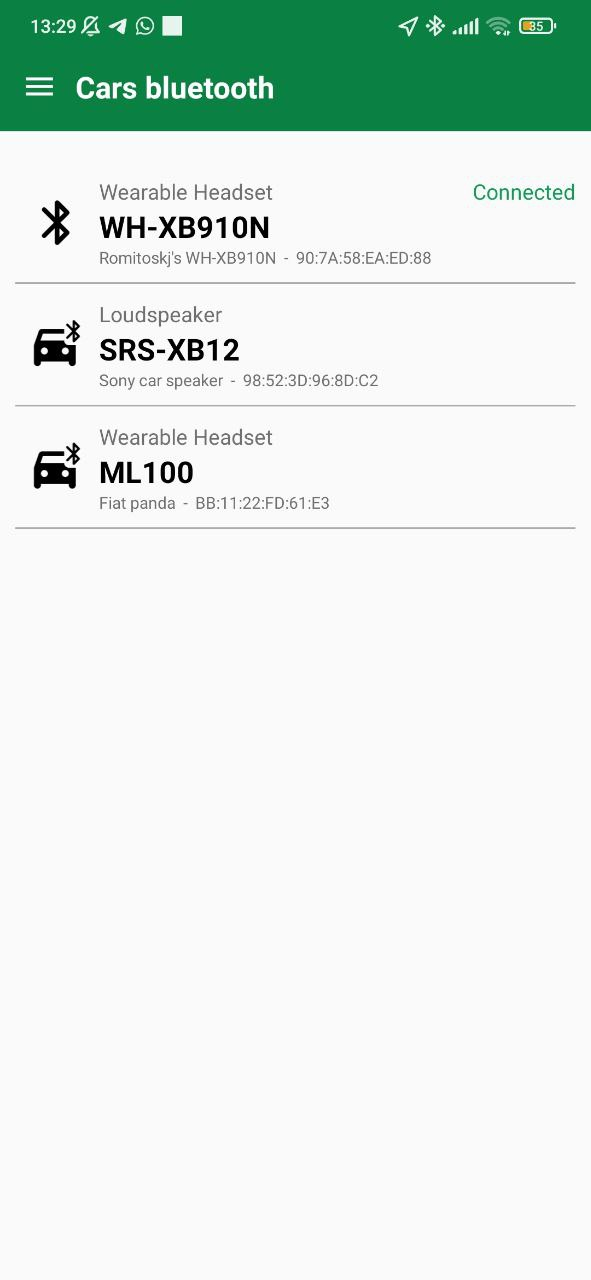
\includegraphics[width=0.9\linewidth]{images/bluetooth_activity.jpg}
    \caption{Interfaccia utente del sensore Bluetooth}
    \label{fig:bluetooth_activity}
\end{wrapfigure}
sia \textit{update} che \textit{collect} prendono in input un oggetto di tipo SensorData, il quale ha lo scopo di serializzare i dati relativi allo stato del sensore, come riportato in un esempio qui sopra, e inviarli al server tramite la web API definita dal backend nella maniera descritta nel paragrafo \ref{chap:sensorData}. Come tutti per tutti i sensori vengono inviati i dati relativi alla confidenza, all'azione compiuta dall'utente e il timestamp che indica il momento in cui essi sono stati calcolati. In aggiunta a ciò nel campo data il sensore Bluetooth serializza il suo stato, nello specifico indica se il Bluetooth dello smartphone è acceso o meno e in caso affermativo invia la lista dei dispositivi ad esso connessi. Inoltre per ogni dispositivo viene indicato il nome, l'alias, la classe Bluetooth, se è una macchina o meno e il numero di connessioni effettuate.

\section{La presentazione dei dati}
Come per la prima applicazione sviluppata è stata creata un'interfaccia utente visibile in figura \ref{fig:bluetooth_activity} e accessibile dal menu laterale di GeneroCity. Essa consente di visualizzare le macchine salvate nella mappa \textit{cars} e i dispositivi connessi, il tutto in un unica lista ordinata in modo da avere i dispositivi connessi in alto e successivamente tutti gli altri ordinati in base al numero di connessioni effettuate, quindi le macchine con più connessioni appariranno più in alto nella lista. Inoltre per ogni dispositivo è stata aggiunta un'icona che aiuta l'utente a distinguere se si tratta di una macchina o meno. Tutto ciò è stato implementato utilizzando un \textit{BluetoothDeviceAdapter} in maniera simile a quanto descritto nel paragrafo \ref{ref:presentation} di cui è stato definito il metodo onDeviceUpdate in modo da fondere la lista dei dispositivi connessi e delle macchine ottenute dal Controller e ordinarle come descritto prima. Questo metodo viene quindi registrato come listener del Controller in modo da aggiornare l'interfaccia ogni volta che esso cambia stato. La definizione del BluetoothDeviceAdapter viene riportata qui sotto.
\begin{minted}[
framesep=2mm,
linenos,
bgcolor=LightGray,
breaklines
]{java}
BluetoothDeviceAdapter bluetoothDeviceAdapter = new BluetoothDeviceAdapter(this) {
    @Override
    public void updateDevices() {
        BluetoothController controller = BluetoothController.getInstance(
            BluetoothSensorActivity.this
            );

        Comparator<BluetoothDevice> deviceComparator = Comparator.comparing(
                        (BluetoothDevice bluetoothDevice) -> bluetoothDevice.isConnected(context),
                        Comparator.reverseOrder()
                )
                .thenComparing(BluetoothDevice::getConnectionCount, Comparator.reverseOrder())
                .thenComparing(BluetoothDevice::getLastConnection, Comparator.reverseOrder());

        devices = Stream.concat(controller.getCars().stream(), controller.getConnectedDevices().stream())  // merge cars and connected devices
                .distinct()  // remove duplicates
                .sorted(deviceComparator)  // sort by connection status, connection count and last connection
                .collect(Collectors.toList());

        notifyDataSetChanged();
    }
};
\end{minted}


\section{Il testing del sensore}
Sia durante lo sviluppo del sensore sia dopo di esso sono state effettuate delle prove con smartphone differenti ed alcuni modelli di macchine con autoradio dotate di Bluetooth, ciò allo scopo di verificare il corretto funzionamento del sensore Bluetooth. Esse sono state effettuate tutte in sicurezza, dato che per questo sensore è necessario solamente instaurare una connessione tra la macchina e uno smartphone senza la necessita di mettersi effettivamente alla guida. In particolare è stato importante controllare che tutte le macchine venissero rilevate, indipendentemente se attraverso la classe Bluetooth o il nome del dispositivo, e che la confidenza aumentasse sempre coerentemente al numero di connessioni effettuate con la stessa auto. È stato possibile avere un riscontro dei risultati attraverso l'interfaccia utente descritta precedentemente, visualizzando i log forniti dall'applicazione e analizzando i dati che sono stati inseriti nel database attraverso l'utilizzo della web API. In seguito a questi test si è dimostrato che il sensore è in grado di effettuare il suo compito, ossia di determinare automaticamente quando l'utente si trova alla guida della propria auto basandosi sulla tecnologia Bluetooth. Inoltre questa fase ha confermato l'integrazione completa del sensore Bluetooth con il sistema di GeneroCity.